\documentclass[sutton_barto_notes.tex]{subfiles}
\begin{document}

\newpage
\section{Off-policy Methods with Approximation}

\begin{itemize}
\item The extension to function approximation is significantly different and difficult for off-policy learning, than it is for on-policy learning
\item tabular off-policy methods
\begin{itemize}
	\item extend to semi-gradient algorithms
	\item do not converge robustly compared to when they under on-policy trainings.
\end{itemize}
\item convergence problem
\item notion of learnability
\item introduce new algorithms for off-policy case with stronger convergence
\item off-policy
\begin{itemize}
	\item prediction case: both $\pi$ and $b$ are static and given, we learn either $\hat{v} \approx v_\pi$ or $\hat{q}\approx q_\pi$.
	\item control case: $\hat{q}$ are learned, $\pi$ and $b$ changes during learning.)
\end{itemize}
\item \textbf{challenges}
\begin{itemize}
\item (mismatched) target of the update (solution: semi-gradients, importance sampling)
\item (mismatched) distribution of the updates, like distribution shift in offline RL? (solution: (1) importance sampling; (2) true gradient methods)
\end{itemize}
\end{itemize}

\subsection{Semi-gradient Methods}

To address "mismatched target of the update", we change from tabular form to \textbf{semi-gradient form}: replace (update to array/table $V,Q$) $\rightarrow$ (update to weight vector $\bm{w}$ using $\hat{v},\hat{q}$ and its gradient).

\paragraph{semi-gradient reminder (chap 9.3)}

Semi-gradient arise when it is not possible to compute the true gradient.

We use gradient to update the weight vector $\bw$, in approximation methods to produce the values $\hat{v}(S_t, {\bw}_t$.

To minimize the error on observed samples, we have a \textit{true gradient} of the form:
$$ \mathbf{w}_{t+1} = \mathbf{w}_t - \alpha \big[v_{\pi}(S_t) - \hat{v}(S_t, \mathbf{w}_t)\big] \nabla \hat{v}(S_t, \mathbf{w}_t) $$

However, we don't have the true target value $v_\pi(S_t)$, so we use an estimate $U_t$:
$$\mathbf{w}_{t+1} = \mathbf{w}_t - \alpha \big[U_t - \hat{v}(S_t, \mathbf{w}_t)\big] \nabla \hat{v}(S_t, \mathbf{w}_t) $$

If $U_t$ is \textbf{unbiased}, like MC ($U_t = G_t$), then we have \textbf{convergence guarantees}.

If $U_t$ is \textbf{biased}, like (TD, DP that bootstrap on estimates, which need the current ${\bw}_t$, then we have \textbf{semi-gradient} methods. The optimized value ($\bw_t$) is also used in the target to compute the gradient.

\paragraph{how semi-gradients solve challenge 1?}
Chapter 7 described off-policy algorithms, we convert them to semi-gradient form to get full update.

on-policy TD(0):
$$ \mathbf{w}_{t+1} = \mathbf{w}_t + \alpha \delta_t \nabla\hat{v}(S_t, \mathbf{w}_t) $$
off-policy TD(0):
$$ \mathbf{w}_{t+1} = \mathbf{w}_t + \alpha \delta_t \rho_t \nabla\hat{v}(S_t, \mathbf{w}_t) $$
where $\delta_t$ depends on episodic / discounted / continuous (average reward) problems.

For action-values, the one-step algorithm is semi-gradient Expected SARSA:
$$ \mathbf{w}_{t+1} = \mathbf{w}_t + \alpha \delta_t \nabla\hat{q}(S_t, A_t, \mathbf{w}_t) $$
with
\begin{align}
\delta_t & = R_{t+1} + \gamma \sum_a \pi(a|S_{t+1}) \hat{q}(S_{t+1}, a, \mathbf{w}) - \hat{q}(S_t, A_t, \mathbf{w}) \quad \quad \quad \quad \quad \mathrm{(episodic)} \label{eq:11.6}\tag{11.6}\\
\delta_t & = R_{t+1} + \bar{R}_t + \sum_a \pi(a|S_{t+1}) \hat{q}(S_{t+1}, a, \mathbf{w}) - \hat{q}(S_t, A_t, \mathbf{w}) \quad \quad \quad \mathrm{(continuing)} \label{eq:11.7}\tag{11.7}
\end{align}
Notice that we don't have IS here!
\begin{itemize}
\item In the tabular case, it's normal because Expected SARSA's last step is not sampled like SARSA. It is a sum over all possible actions, weighted over the \textbf{target} policy, not the behavior policy, so there is no need for importance sampling
\item with FA, it's less clear, because different $q$ values may contribute to the same approximation, this is ongoing research
\item n-step Expected SARSA (with IS):
\end{itemize}
$$ \mathbf{w}_{t+1} = \mathbf{w}_{t+n-1} + \alpha \rho_{t+1} ... \rho_{t+n-1} [G_{t:t+n} - \hat{q}(S_t, A_t, \mathbf{w}_{t+n-1})] \nabla\hat{q}(S_t, A_t, \mathbf{w}_{t+n-1}) $$
where $G_{t:t+n}$ is defined differently for episodic and continuing case (continuing cases use average returns).
\begin{itemize}
\item The n-step backup tree algorithm doesn't use IS. Its semi-gradient form:
\end{itemize}
\begin{align}
\mathbf{w}_{t+1} & = \mathbf{w}_{t+n-1} + \alpha [G_{t:t+n} - \hat{q}(S_t, A_t, \mathbf{w}_{t+n-1})] \nabla\hat{q}(S_t, A_t, \mathbf{w}_{t+n-1}) \label{eq:11.9}\tag{11.9}\\
G_{t:t+n} & = \hat{q}(S_t, A_t, \mathbf{w}_{t-1}) + \sum_{k=t}^{t+n-1} \delta_k \prod_{i=t+1}^k \gamma \pi(A_i|S_i) \label{eq:11.10}\tag{11.10}
\end{align}

\subsection{Examples of Off-policy Divergence}

First example: $w$ -> $2w$

Second example: Biard's counterexample (semi-gradient off-policy TD/DP diverges)

The examples illustrate that, \textbf{with off-policy learning, semi-gradient methods will diverge}.

The Biard's counterexample, using the simplest bootstrapping method (DP), along with the simplest form of parametrization (linear), show that the combination of bootstrapping and function approximation can be unstable in the off-policy case. A Q-learning version of Baird’s example also exists. For Q-learning though, we can guarantee convergence if the behaviour policy is sufficiently close to the target policy, such as $\varepsilon$-greedy policies.

How to find stability then? The truth is, we don’t really have theoretical guarantees for methods that extrapolate information from observation, such as neural network approximators. We do have stability guarantees for function approximation methods that do not extrapolate, like nearest neighbor averagers, but these methods are not as popular as neural networks.

\subsection{Deadly triad of divergence}

\begin{itemize}
\item function approximation
\item bootstrapping
\item off-policy training
\end{itemize}

Instability can be avoided if we remove one of the elements.
\begin{itemize}
\item FA cannot be given up. Need it for large state spaces
\item Doing w/o bootstrapping is possible, but with a loss in computational efficiency (like MC)
\item Maybe off-policy is the best to drop (SARSA instead of Q-learning)
\item There is no satisfactory solution because we still need off-policy to do model planning
\end{itemize}

\subsection{Linear Value-function Geometry}


\begin{figure}[h!]
    \centering
    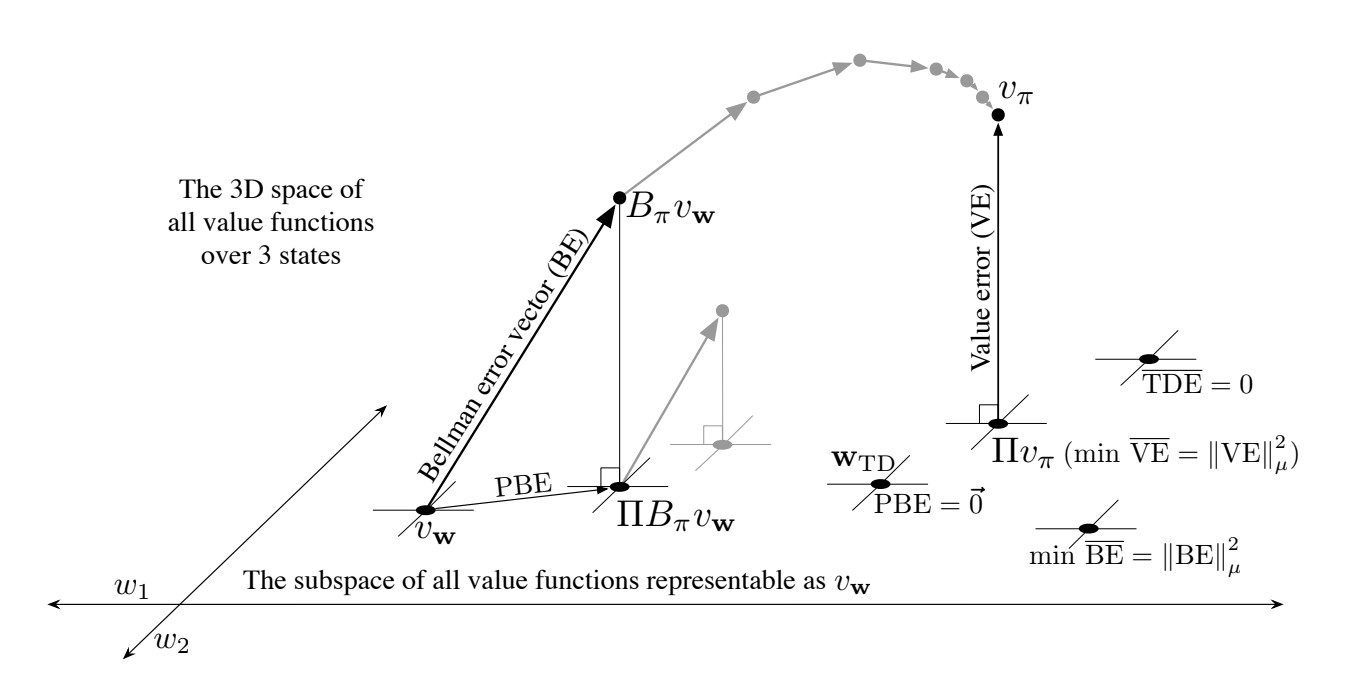
\includegraphics[width=0.9\textwidth]{bellman_error.png}
    \caption{ Geometry of linear FA (see book note) }
\end{figure}

\newpage
Distance between value functions
$$ \| v \|^2_\mu \doteq \sum_{s \in \cS} \mu(s) v(s)^2 $$
\textbf{Value Error} norm
$$ \overline{VE}(\bw) = \| v_{\bw} - v_\pi \|^2_\mu$$
\textbf{Projection Operation} $\prod$
$$ \prod v \doteq v_{\bw} \quad\quad {\bw} = \arg\min_{ {\bw} \in \bR^d } \| v - v_{\bw} \|^2_\mu $$
\textbf{Bellman error} $\bar{\delta}_{\bw}$ at state $s$ is a measure of the distance between $v_\pi$ and $v_{\bw}$
\begin{align*}
\bar{\delta}_{\mathbf{w}} & \doteq \Big( \sum_a \pi(a|s) \sum_{s', r} p(s', r| s, a) [r + \gamma v_{\mathbf{w}}(s')]\Big) - v_{\bw}(s) \\
 & = \mathbb{E}_{\pi} [R_{t+1} + \gamma v_{\mathbf{w}}(S_{t+1}) - v_{\mathbf{w}}(S_{t}) | S_t = s, A_t \sim \pi ]
\end{align*}
\textbf{Mean Square Bellman Error}
$$ \overline{BE}(\mathbf{w}) = \| \bar{\delta}_{\mathbf{w}} \|_{\mu}^2 $$
\textbf{Mean Square Projected Bellman Error}
$$ \overline{PBE}(\mathbf{w}) = \| \Pi\bar{\delta}_{\mathbf{w}} \|_{\mu}^2 $$
\textbf{Mean Square TD Error}
$$ \overline{TDE} = {\bE}_b [ \rho_t \delta_t^2 ] $$
where
$$ \delta_t = R_{t+1} + \gamma \hat{v}(S_{t+1}, \mathbf{w}_t) - \hat{v}(S_t, \mathbf{w}_t) $$
\textbf{Mean Square Return Error}
$$ \overline{RE} = \bE [ (G_t - \hat{v}(S_t, \bw) )^2 ] = \overline{VE} (\bw) + \bE [ ( G_t - v_\pi(S_t) )^2 ] $$


Summary
\begin{itemize}
\item the \textbf{Bellman operator} $B_\pi$ takes the value function out of the $d$-dimensional subspace and have to be projected back to be followed (PBE)
\item zero $\overline{PBE}$ = TD fixed point
\end{itemize}

\subsection{Gradient Descent in the Bellman Error}

\begin{itemize}
\item In true SGD, updates are made in the direction of the negative gradient and in expectation go downhill, giving good convergence properties
\item Only MC uses true SGD, semi-gradients with bootstraping do not
\item To apply SGD we need an objective function, and this section explore objective functions based on the Bellman Error discussed in the previous section
\end{itemize}


\paragraph{First approach}: minimize $\overline{TDE}$

This converges, but not necessarily converge to a desirable place.

It also has larger TD error. so minimizing $\overline{TDE}$ is not good.

\paragraph{Second approach}: minimize Bellman error (if hte exact values are learned, the Bellman error = 0)

It gives the \textbf{residual gradient algorithm}.

It has good convergence and minimizes the BE. But it seems to converge to wrong values in FA. So minimizing BE is not good.

\subsection{The Bellman Error is not learnable}

\begin{itemize}
\item $\overline{BE}$ itself is not learnable. It can be computed from MDP, but not directly from data.
\item $\overline{VE}$ itself is not learnable. However, its optimizer is.
\item $\overline{PBE}$ and $\overline{TDE}$ are learnable from data.
\end{itemize}

\begin{figure}[h!]
    \centering
    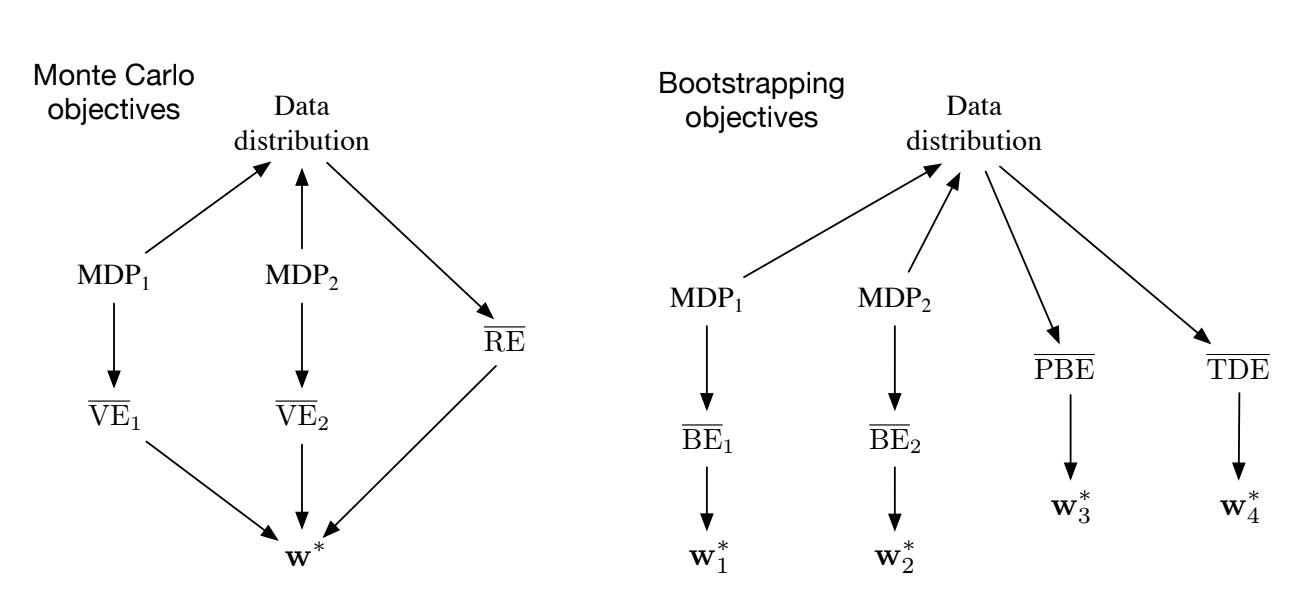
\includegraphics[width=0.9\textwidth]{objectives_summary.png}
    \caption{ Objectives Summary }
\end{figure}

\newpage
\subsection{Gradient TD methods}

Since semi-gradient don't have good convergence guarantee, we now consider \textbf{true SGD} methods to minimize $\overline{PBE}$.

\begin{itemize}
\item in the linear case, there is always a solution, the TD fixed point ${\bw}_TD$, at which $\overbrace{PBE} = 0$.
\item Least-Squares method gives a $O(d^2)$ solution, and we want a $O(d)$ solution with SGD
\item still assume linear FA
\item 
\end{itemize}

\paragraph{Projection matrix}
 
For a linear function approximator, the projection operation is linear, and can be represented by an $|\mathcal{S}| \times |\mathcal{S}|$ matrix: 
\begin{align}
\Pi \doteq \mathbf{X} (\mathbf{X}^{\top} \mathbf{D} \mathbf{X})^{-1} \mathbf{X}^{\top} \mathbf{D} \label{eq:11.21}\tag{11.21}
\end{align}

 Where: 
\begin{itemize}
\item $\mathbf{D}$ denotes the diagonal $|\mathcal{S}| \times |\mathcal{S}|$ with the $\mu(s)$ values on the diagonal ($\mu(s)$ represents how much we care about state $s$ (see chap 9.2)
\item $\mathbf{X}$ denotes the $|\mathcal{S}| \times d$ matrix whose rows are the feature vectors $\mathcal{x}(s)^{\top}$ for each state $s$. 
\end{itemize}

 Using these matrices, the squared norm of a vector can be written as: 

\begin{align}
\|v\|_{\mu}^2 = v^{\top} \mathbf{D} v \label{eq:11.22}\tag{11.22}
\end{align}

\paragraph{Objective formulation}  
Then we can rewrite the $\overline{PBE}$ objective in matrix terms. 

 
\begin{align}
\overline{PBE}(\mathbf{w}) & = ||\Pi \bar{\delta}_{\mathbf{w}}||^2_{\mu} \label{eq:11.23}\tag{11.23}\\
 & = (\Pi \bar{\delta}_{\mathbf{w}})^{\top} \mathbf{D} \Pi \bar{\delta}_{\mathbf{w}} \label{eq:11.24}\tag{11.24}\\
 & = \bar{\delta}^{\top}_{\mathbf{w}} \mathbf{D} \mathbf{X} (\mathbf{X}^{\top} \mathbf{D} \mathbf{X})^{-1} \mathbf{X}^{\top} \mathbf{D} \bar{\delta}_{\mathbf{w}} \label{eq:11.25}\tag{11.25}\\
 & = (\mathbf{X}^{\top} \mathbf{D} \bar{\delta}_{\mathbf{w}})^{\top} (\mathbf{X}^{\top} \mathbf{D} \mathbf{X}){-1} (\mathbf{X}^{\top} \mathbf{D} \bar{\delta}_{\mathbf{w}}) \label{eq:11.26}\tag{11.26}
\end{align} 

 Explanation: 
\begin{itemize}
\item \ref{eq:11.23} is the $\overline{PBE}$ definition (\ref{eq:11.14}) 
\item \ref{eq:11.24} uses \ref{eq:11.22} 
\item \ref{eq:11.25} uses $\Pi$ definition (\ref{eq:11.21}) and identity $\Pi^{\top} \mathbf{D} \Pi = \mathbf{D} \mathbf{X} (\mathbf{X}^{\top} \mathbf{D} \mathbf{X})^{-1} \mathbf{X}^{\top} \mathbf{D}$ 
\end{itemize}

 \paragraph{Gradient}  
The gradient with respect to $\mathbf{w}$ is: 
\begin{align}
\nabla \overline{PBE}(\mathbf{w}) = 2 \nabla [\mathbf{X}^{\top} \mathbf{D} \bar{\delta}_{\mathbf{w}}]^{\top} (\mathbf{X}^{\top} \mathbf{D} \mathbf{X}){-1} (\mathbf{X}^{\top} \mathbf{D} \bar{\delta}_{\mathbf{w}}) \label{eq:11.27}\tag{11.27}
\end{align}

\begin{itemize}
\item Turn that into an SGD method: sample something on every timestep that has this quantity on expectation 
\item If $\mu$ is the distribution of the states visited under the behaviour policy, 
\item All three factors can be expressed in terms of expectations under this distribution (details for each factors in the book) 
\end{itemize}
 End result: 
\begin{align}
\nabla \overline{PBE}(\mathbf{w}) = 2 \mathbb{E}[\rho_t(\gamma \mathbf{x}_{t+1} -  \mathbf{x}_t)\mathbf{x}_t^{\top}] \; \mathbb{E}[\mathbf{x}_t \mathbf{x}_t^{\top}]^{-1} \; \mathbb{E}[\rho_t \delta_t \mathbf{x}_t] \label{eq:11.28}\tag{11.28}
\end{align}


\begin{itemize}
\item still the first and last expressions are not independant (same sample vector $\mathbf{x}_{t+1}$) (-> biased) 
\item we could estimate the 3 factors separately and then combine them but it would be too computationally expensive 
\item If 2 out of 3 factors are estimated and stored then we sample the last -> still $O(d^2)$ 
\end{itemize}

 \textbf{Gradient-TD}  
\begin{itemize}
\item store the <em>product</em> of the two last factors (product of $d \times d$ matrix and $d$ vector so we get a $d$ vector) 
\item this product is a $d$-vector, like $\mathbf{w}$ itself. We call it $\mathbf{v}$: 
\end{itemize}

\begin{align}
\mathbf{v} \approx \mathbb{E}[\mathbf{x}_t \mathbf{x}_t^{\top}]^{-1} \; \mathbb{E}[\rho_t \delta_t \mathbf{x}_t] \label{eq:11.29}\tag{11.29}
\end{align}
\begin{itemize}
\item (linear supervised learning) solution to a linear least squares problem that tries to approximate $\rho_t \delta_t$ from experience 
\item Standard SGD method for finding the $v$ that minimizes the expected squared error is the Least Mean Square (LMS): 
\end{itemize}
\begin{align}
\mathbf{v}_{t+1} = \mathbf{v}_t + \beta \rho_t (\delta_t - \mathbf{v}_t^{\top} \mathbf{x}_t) \mathbf{x}_t \label{eq:11.30}\tag{11.30}
\end{align}

\begin{itemize}
\item $\beta > 0$ is the step size parameter 
\item $\rho_t$ importance sampling ratio 
\item $O(d)$ storage and computation 
\end{itemize}
 \paragraph{GTD2} 
Given $\mathbf{v}$ (\ref{eq:11.30}) we can update our main parameter $\mathbf{w}$ using SGD: 
\begin{align}
\mathbf{w}_{t+1} & = \mathbf{w}_{t} - \frac{1}{2} \alpha \nabla \overline{PBE}(\mathbf{w}_{t}) \label{eq:11.31}\tag{11.31}\\
 & = \mathbf{w}_{t} - \frac{1}{2} \alpha 2 \mathbb{E} [\rho_t(\gamma \mathbf{x}_{t+1} - \mathbf{x}_{t}) \mathbf{x}_{t}^{\top}] \mathbb{E}[\mathbf{x}_{t} \mathbf{x}_{t}^{\top}]^{-1} \mathbb{E}[\rho_t \delta_t \mathbf{x}_{t}] \label{eq:11.32}\tag{11.32}\\
 & = \mathbf{w}_{t} + \alpha \mathbb{E} [\rho_t(\mathbf{x}_{t} - \gamma \mathbf{x}_{t+1}) \mathbf{x}_{t}^{\top}] \mathbb{E}[\mathbf{x}_{t} \mathbf{x}_{t}^{\top}]^{-1} \mathbb{E}[\rho_t \delta_t \mathbf{x}_{t}] \label{eq:11.33}\tag{11.33}\\
  & \approx \mathbf{w}_{t} + \alpha \mathbb{E} [\rho_t(\mathbf{x}_{t} - \gamma \mathbf{x}_{t+1}) \mathbf{x}_{t}^{\top}] \mathbf{v}_t \label{eq:11.34}\tag{11.34}\\
  & \approx \mathbf{w}_{t} + \alpha \rho_t(\mathbf{x}_{t} - \gamma \mathbf{x}_{t+1}) \mathbf{x}_{t}^{\top} \mathbf{v}_t \label{eq:11.35}\tag{11.35}
\end{align} 

 Explanation: 
\begin{itemize}
\item \ref{eq:11.31} is from the general SGD rule 
\item \ref{eq:11.32} is using the gradient $\nabla \overline{PBE}(\mathbf{w})$ from \ref{eq:11.28} 
\item \ref{eq:11.33} is from algebraic arrangements 
\item The approximation made in \ref{eq:11.34} is using the approximation from \ref{eq:11.29} 
\item And we remove the expectation to get \ref{eq:11.35} by sampling 
\end{itemize}

 This algorithm is called GTD2 and in the last step if the inner product $\mathbf{x}_t^{\top} \mathbf{v}_t$ is done first it is $O(d)$ 

 \textbf{TD(0) with gradient correction (TDC), or GTD(0)} 
A better version with more analytic steps between \ref{eq:11.33} and the $\mathbf{v}_t$ substitution gives the following update: 
\begin{align}
\mathbf{w}_{t+1} \approx \mathbf{w}_{t} + \alpha \rho_t(\delta_t \mathbf{x}_{t} - \gamma \mathbf{x}_{t+1} \mathbf{x}_{t}^{\top} \mathbf{v}_t) \label{eq:11.36}\tag{11.36}
\end{align}

 \paragraph{Summary and further reading}   
\begin{itemize}
\item Both GTD2 and TDC involve two learning processes, one for $\mathbf{v}$ and one for $\mathbf{w}$ 
\item asymetrical dependence ($\mathbf{v}$ doesn’t need $\mathbf{w}$ but $\mathbf{w}$ needs $\mathbf{v}$) -> \textbf{cascade} 
\item usually the secondary learning process ($\mathbf{v}$) is faster 
\item Extension to non-linear function approximation: Maei et al 2009 
\item Hybrid TD algorithms 
\item Gradient-TD combined with proximal methods and control variates -> Mahadevan et al 2014 
\end{itemize}

\subsection{Emphatic TD methods}

\begin{itemize}
\item In this section we explore a major strategy for obtaining a cheap and efficient method for off-policy learning with function approximation 
\item linear semi-gradient methods are stable under on-policy distribution (chap 9.4)
\item it works because there is a match between the on-policy state distribution and the state-transition probabilities under the target policy 
\item we don’t have this match anymore in off-policy! 
\textbf{Solution}: reweight the states, emphasizing some and de-emphasizing others, so as to return the distribution of updates to the on-policy distribution 
\end{itemize}

 There is no unique “on-policy distribution” 

 The one-step Emphatic-TD algorithm for learning episodic state values is defined by: 

 
\begin{align}
\delta_t & = R_{t+1} + \gamma \hat{v}(S_{t+1}, \mathbf{w}_t) - \hat{v}(S_t, \mathbf{w}_t) \label{eq:11.37}\tag{11.37}\\
\mathbf{w}_{t+1} & = \mathbf{w}_t + \alpha M_t \rho_t \delta_t \nabla \hat{v}(S_t, \mathbf{w}_t) \label{eq:11.38}\tag{11.38}\\
M_t & = \gamma \rho_{t-1} M_{t-1} + I_t \label{eq:11.39}\tag{11.39}
\end{align} 

\begin{itemize}
\item $I_t$, the \textbf{interest}, is arbitraty 
\item $M_t$, the \textbf{emphasis}, is init with $M_{t-1} = 0$ 
\item In Baird’s counterexample, this algorithm converges in theory, but in practice the variance is so high that it’s impossible to use 
\end{itemize}

\subsection{Reducing the variance}

\begin{itemize}
\item off-policy variance > on-policy variance by design 
\item policy ratios ($\rho$):
    \begin{itemize}
    \item 1 in expected value 
    \item can be as low as 0 in practice 
    \item successive importance sampling ratios are not correlated, so their product is always one 
    \end{itemize}
   
\item these ratios multiply the step size in SGD methods so the impact of their variance can be huge 
\item things that can help:
    \begin{itemize}
    \item momentum 
    \item Polyak-Ruppert averaging 
    \item adaptively setting separate step-sizes for different components of the parameter vector (w) 
    \item weighted importance sampling (chap 5) is well-behaved but still tricky to adapt to function approximation (Mahmood and Sutton 2015) 
    \item off-policy without importance sampling (Munos, Stepleton, Harutyunyan, and Bellemare (2016) and Mahmood, Yu and Sutton (2017)) 
    \end{itemize}
   
\end{itemize}

\subsection{Summary}

\begin{itemize}
\item Tabular Q-learning makes off-policy learning seem easy, as its extensions Expected Sarsa and Tree Backup algorithm 
\item Extension to function approximation, even linear, is tricky 
\item SGD in the Bellman Error (BE) doesn’t really work because it’s not learnable 
\item Gradient-TD methods performs SGD in the <em>projected</em> Bellman error 
\item Emphatic-TD methods try to reweight updates to be closer to on-policy setting 
\end{itemize}







\end{document}